\documentclass{standalone}
\usepackage{tikz}
\usepackage{ctex,siunitx}
\usepackage{tkz-euclide}
\usepackage{amsmath}
\usetikzlibrary{patterns, calc}
\usetikzlibrary {decorations.pathmorphing, decorations.pathreplacing, decorations.shapes,}
\begin{document}
\small
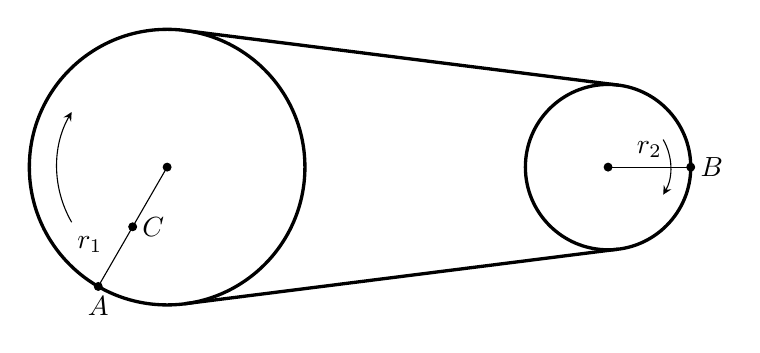
\begin{tikzpicture}[>=stealth, scale=0.7]
  \tkzDefPoints{0/0/O,8/0/A,2.5/0/B,9.5/0/C}
  \tkzDefSimilitudeCenter[ext](O,B)(A,C)
  \tkzGetPoint{J}
  \tkzDefLine[tangent from = J](O,B)
  \tkzGetPoints{F}{G}
  \tkzDefLine[tangent from = J](A,C)
  \tkzGetPoints{F'}{G'}
  \draw [very thick](0,0)  circle [radius=2.5];
  \draw [very thick](8,0)  circle [radius=1.5];
  \draw [->](210:2) arc (210:150:2);
  \draw [->](9,.5) arc (30:-30:1);
  \draw (0,0)--(240:2.5)node [pos=0.8,above left]{$r_1$};
  \draw (8,0)--node [above]{$r_2$}(9.5,0);
  \draw [fill=black] (240:2.5) circle (2pt)node [below]{$A$};
  \draw [fill=black] (240:1.25) circle (2pt) node [right]{$C$};
  \draw [fill=black] (0,0) circle (2pt) ;
  \draw [fill=black] (8,0) circle (2pt) ;
  \draw [fill=black] (9.5,0) circle (2pt) node [right]{$B$} ;
  \draw [very thick] (F)--(F');
  \draw [very thick] (G)--(G');
\end{tikzpicture}
\end{document}